\section{Theorie}

\subsection{Allgemeines zur Compton-Streuung}  

\begin{flushleft}
    Der Compton-Effekt ist ein Phänomen bei dem eine Verschiebung der Wellenlängen von Elektronen stattfindet, wenn diese gestreut werden.
    In diesem Versuch wird diese Compton-Wellenlänge durch eine sogenannte indirekte Methode bestimmt. 
    Indirekt weil Röntgenstrahlen zur Hilfe benutzt werden.
    Diese Röntgenstrahlen werden auf beispielsweise auf ein Plexiglasquader gestreut, und durch das Transmissionsverhalten die Compton-Wellenlänge bestimmt.
    Wichtig hierbei ist, dass die Streuung der Röntgenstrahlen auf zwei verschiedene Weisen stattfinden kann, und zwar kohärent und inkohärent.
    Die kohärente Streuung, auch Compton-Effekt genannt, ist eine klassisch inelastische Streuung und die inkohärente Streuung eine elastische Frequenzverschobene Streuung.
    Bei dem Compton-Effekt wird ein Photon auf ein Elektron geschossen, wobei das Photon ein Teil seiner Energie an das Elektron abgibt, dadurch seine Wellenlänge zu einer längeren verschoben wird und um den Winkel $\theta$ verschoben wird.
    Die Berechnung der Verschiebung wird durch 
\end{flushleft}

\begin{equation}
    \increment \lambda = \frac{h}{m_{\text{e}}c}\,(1 - \cos(\theta) ) \label{1}
\end{equation}

\begin{flushleft} 
    veranschaulicht.
    Der erste Teil mit $\frac{h}{m_{\text{e}}c}$ ist die Konstante $\lambda_{\text{c}}$, bzw. die Compton-Wellenlänge des Elektrons. 
    Dabei fällt auf je kleiner die Energie des Photons ist, desto länger ist die Wellenlänge.
    Veranschaulicht wird der Compton-Effekt in Abbildung \ref{Abbildung1}.
\end{flushleft}

\begin{figure}[H]       
    \centering
    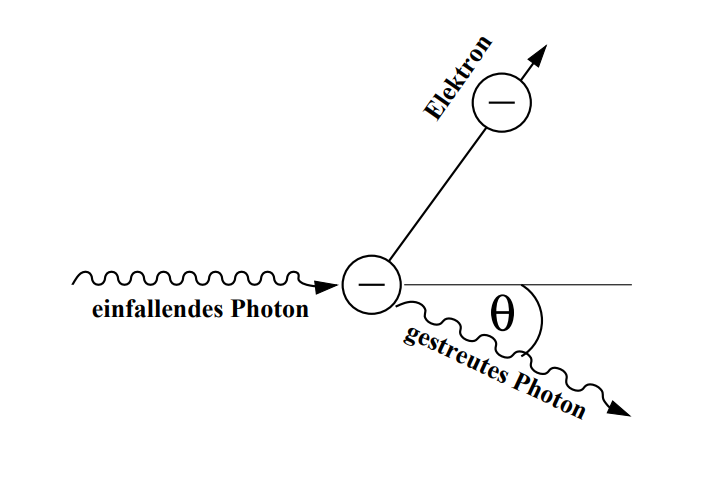
\includegraphics[height=50mm]{bilder/comptoneff.png}
    \caption{Der Compton-Effekt verbildlicht \cite{a1}.\label{Abbildung1} }
\end{figure}

\begin{flushleft}
    Die Wellenlängenverschiebung ist minimal bei $\theta = 0\unit{\degree}$, also $\increment \lambda = 0$  und maximal bei $180\unit{\degree}$, also $\increment \lambda = 2 \cdot \lambda_{\text{c}} $ 
\end{flushleft}

\subsection{Das Erzeugen von Röntgenstrahlung}

\begin{flushleft}
    Um Röntgenstrahlung zu erzeugen werden in einer evakuierten Röhre über eine Glühkathode, Elektronen ausgeschossen.
    Durch die anliegende Spannung zwischen Glühkathode und Anode wird das Elektron auf die Anode hin beschleunigt.
    Beim auftreffen des Elektrons auf der Anode entsteht dann die Röntgenstrahlung. 
    Dies setzt sich aus dem Bremsspektrum und der charakteristischen Röntgenstrahlung des Anodenmaterials zusammen.
    Beim Auftreffen des Elektrons auf der Anode, wird es im Coulombfeld des Atoms abgebremst, wodurch ein Photon ausgesendet wird, mit der Energie die das Elektron im Abbremsvorgang verloren hat.
    Ebenfalls kann auch die gesamte kinetische Energie an das Photon abgegeben werden. 
    Beide Vorgänge werden dem Bremsspektrum zugeordnet und es handelt sich dabei um ein kontinuierliches Spektrum.
    Bei den Übergängen von Energieniveaus der Elektronenschalen entsteht die charakteristische Röntgenstrahlung. 
    Durch Ionisierung des Anodenmaterials können Elektronen aus einer äußeren Schale in eine innere Schale zurückfallen, wenn es von einem Photon getroffen wird.
    Dadurch, dass die Energie des Photons gleich der Energiedifferenz der beiden Energieniveaus ist, besteht das charakteristische Spektrum aus scharfen Linien.
\end{flushleft}

\subsection{Bestimmung der Compton-Wellenlänge}

\begin{flushleft}
    Durch die Transmission und Absorption von Röntgenstrahlung durch Aluminium, kann die Compton-Wellenlänge gut bestimmt werden.
    Transmission hängt von der Wellenlänge ab und wird mit zunehmender Wellenlänge kleiner. 
    Deswegen ist die Transmission der verschobenen Welle auch kleiner als die der einfallende Welle.
    Die Intensität der durch Materie absorbierten Photonen wird gemäß dem Delamber'schen Gesetz um  
\end{flushleft}

\begin{equation}
    I = I_{0}\,e^{-\mu\, d } \label{2}
\end{equation}

\begin{flushleft}
    geschwächt. 
    Der Parameter $d$ steht dabei für die Dicke der Materie und das $\mu$ für den Absorptionskoeffizient. 
    Der Absorptionskoeffizient setzt sich aus dem der Paarbildung, dem des Photoeffekts und dem des Comptoneffektes zusammen  
\end{flushleft}

\begin{align*}
    \mu = \mu_{\text{Paar}} + \mu_{\text{Photo}} + \mu_{\text{Com}}\,.
\end{align*}

\newpage

\subsection{Die Braggsche Reflexion}

\begin{flushleft}
    Eine Möglichkeit die Wellenlänge bzw die Energie der Röntgenstrahlung zu bestimmen, ist durch die Bragg'sche Reflexion.
    Bei der Bragg'schen Reflexion wird ein dreidimensionales Gitter betrachtet in welches Röntgenlicht einfällt. 
    Dabei werden die Photonen an jedem Atom des Gitters gebeugt. 
    Bei dem Glanzwinkel $\alpha$ kommt es zu konstruktiven Interferenz und dieser Winkel kann mit der Bragg'schen Bedingung bestimmt werden.    
\end{flushleft}

\begin{equation}
    2\,d\,\sin(\alpha) = n\, \lambda. \label{3}
\end{equation}

\begin{flushleft}
    Dabei steht $n$ für den Beugungsgrad. 
\end{flushleft}